\section*{Introduction}
\begin{frame}{Motivation}
	\begin{block}{}
	Understanding the implications of time series associated with hydrological variables, such as flow rates or reservoir levels, is essential for hydroelectric generation and the planning of other generation systems in Colombia.
	\end{block}
	\begin{figure}
		\centering
		\begin{subfigure}[b]{0.3\textwidth}
			\centering
			\includegraphics[width=\textwidth, height=3.8cm]{images/irrigation.jpg}
			\caption{Irrigation}
		\end{subfigure}
		\hfill
		\begin{subfigure}[b]{0.3\textwidth}
			\centering
			\includegraphics[width=\textwidth, height=3.8cm]{images/flood_control.jpeg}
			\caption{Flood control}
		\end{subfigure}
		\hfill
		\begin{subfigure}[b]{0.3\textwidth}
			\centering
			\includegraphics[width=\textwidth, height=3.8cm]{images/hydro_gen.jpeg}
			\caption{Hydropower generation}
		\end{subfigure}
		
	\end{figure}
	\begin{block}{\textcolor{myNewColorB}{\textbf{Challenges}}}
	Non-linearities, high stochasticity, and complex water resource patterns.
	\end{block}
	
\end{frame}

\begin{frame}
	\frametitle{The Importance of Hydrological Forecasting}
	\begin{block}{}
	Understanding hydrological processes has become increasingly critical in natural resource management. Suitable forecasting allows the anticipation capacity of extreme hydrological events such as droughts and heavy rainfall.
	\end{block}
	\begin{figure}
		\centering
		\begin{subfigure}[b]{0.45\textwidth}
			\centering
			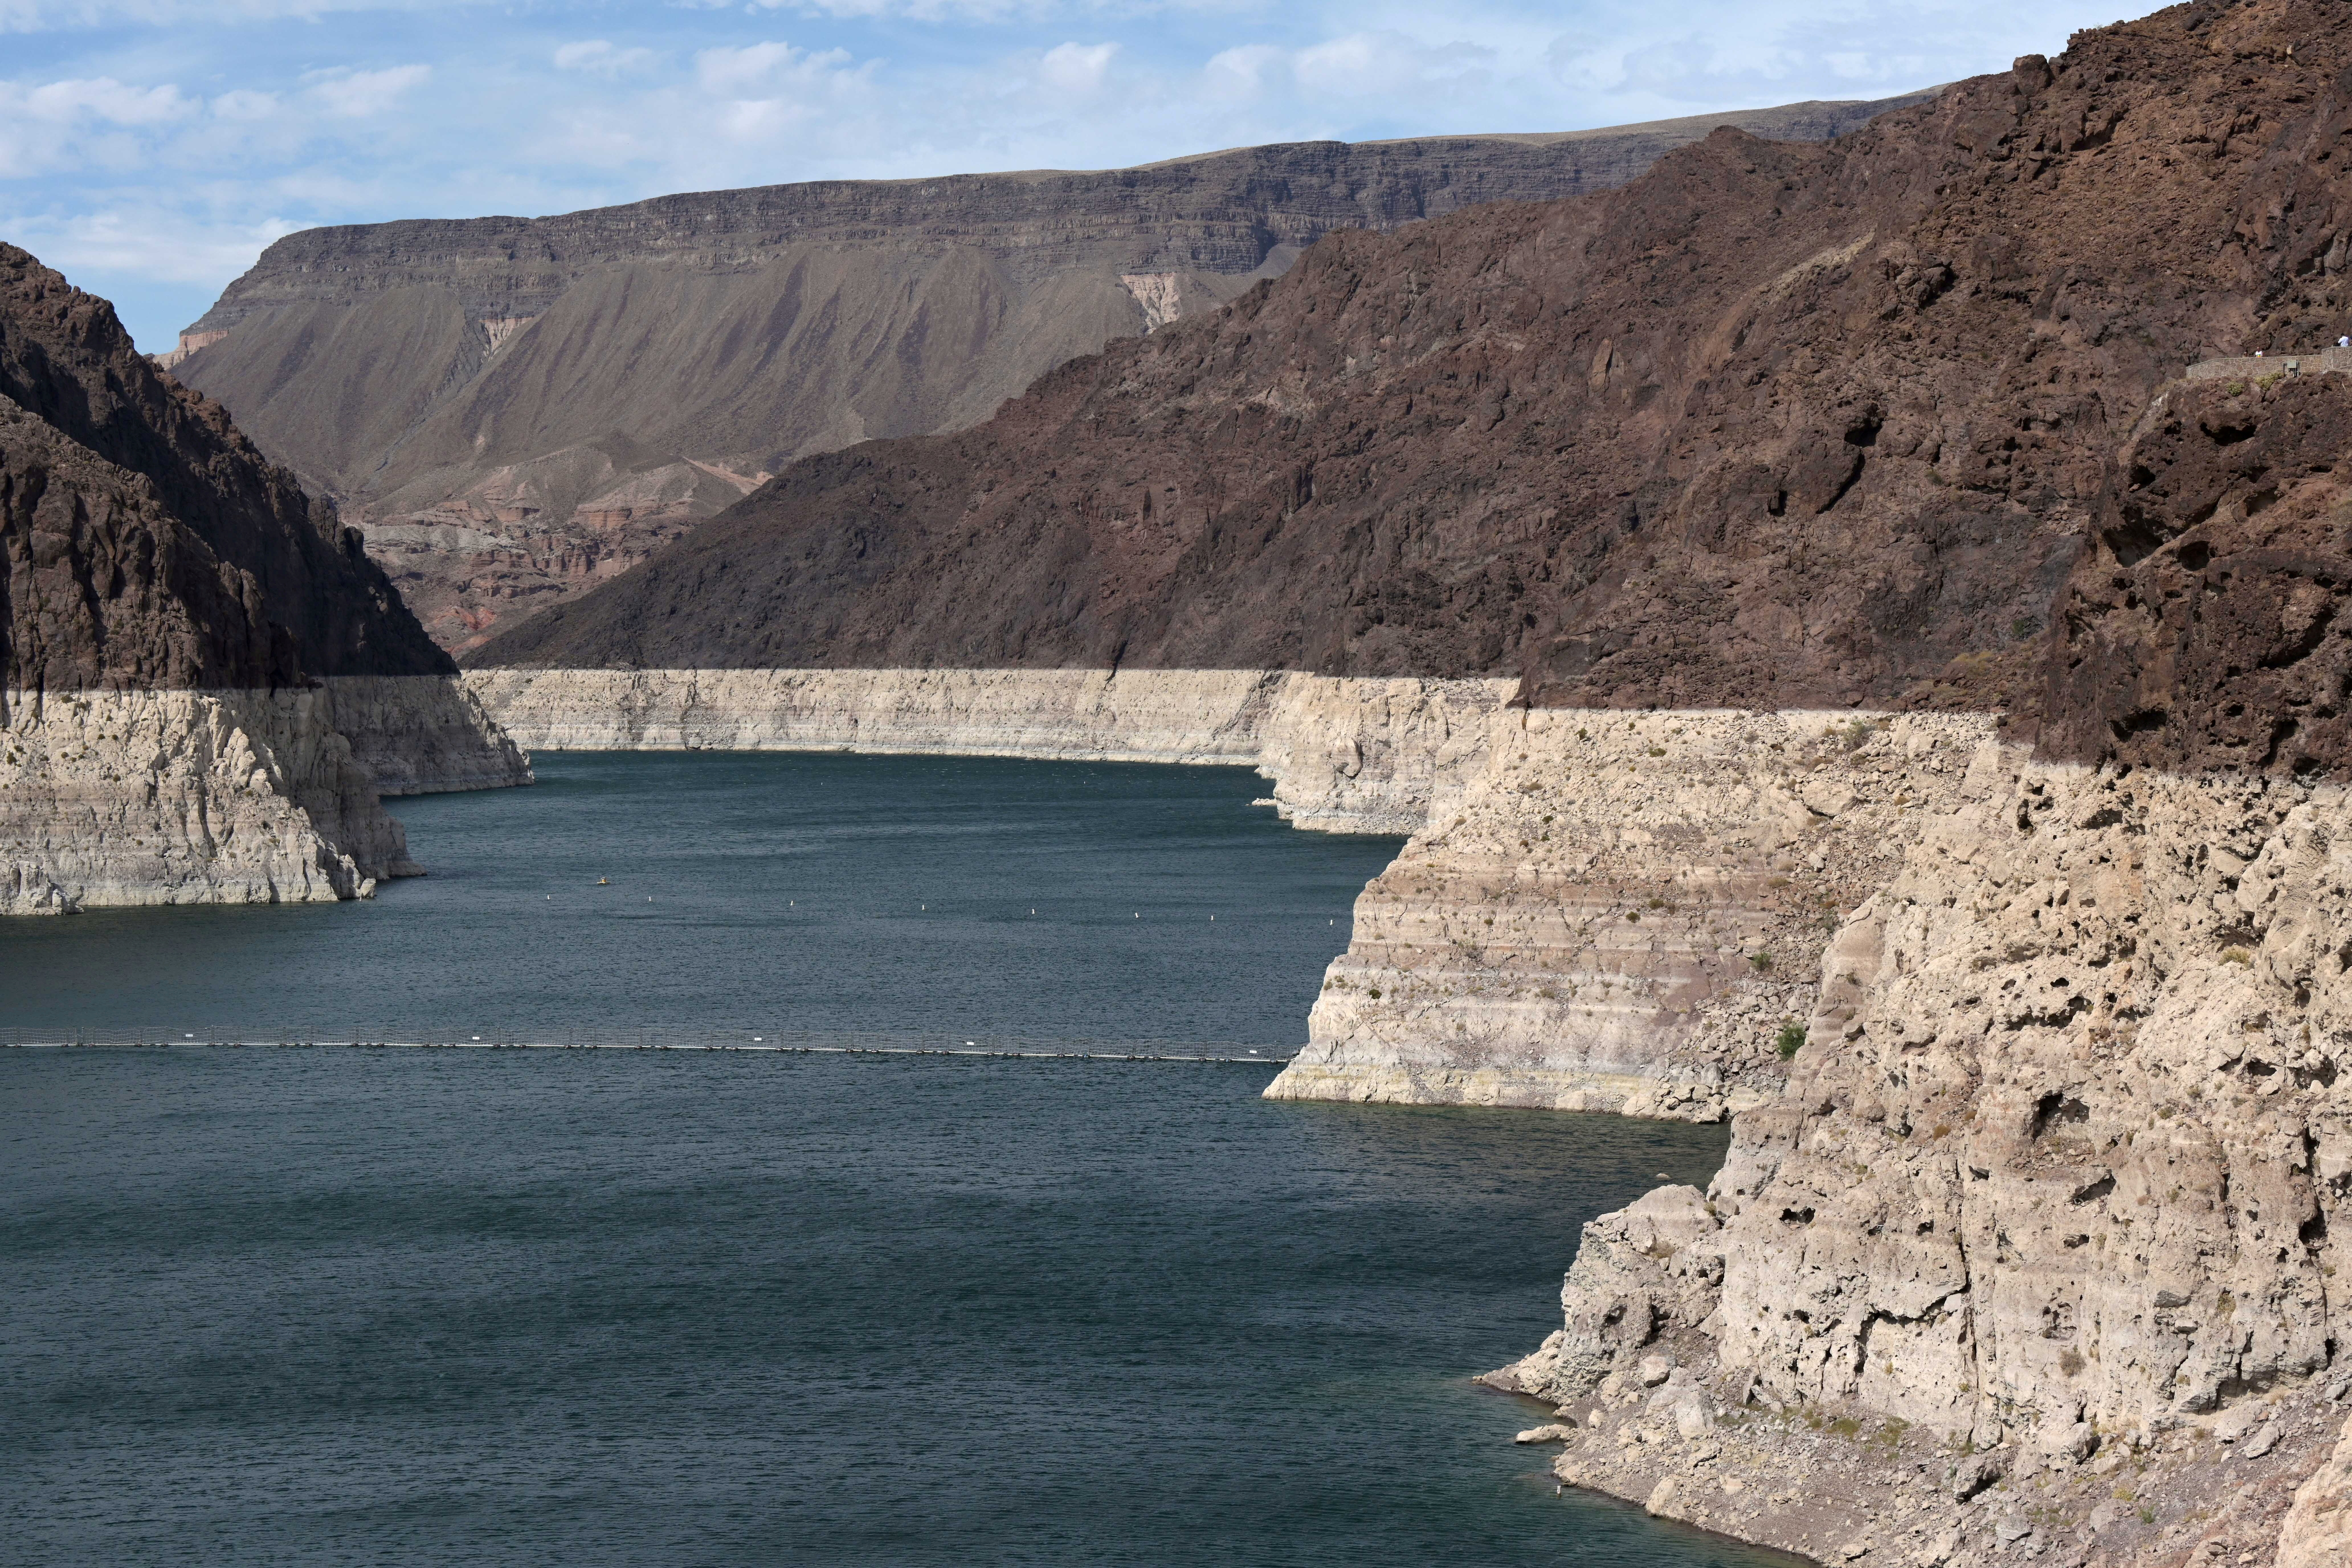
\includegraphics[width=\textwidth, height=4cm]{images/drought.jpg}
			\caption{Drought Condition}
		\end{subfigure}
		\hfill
		\begin{subfigure}[b]{0.45\textwidth}
			\centering
			\includegraphics[width=\textwidth, height=4cm]{images/full_dam.jpg}
			\caption{Full Dam}
		\end{subfigure}
	\end{figure}
	
\end{frame}

\begin{frame}{Problem Statement and Research Question}
	
	\begin{table}[htbp]
		\centering
		\begin{tabular}{l p{1.2cm}p{1.2cm}p{1.2cm}p{1.2cm}p{1.2cm}}
			\toprule
			\textbf{} & \textbf{AR} & \textbf{NN} & \textbf{RNN} & \textbf{LSTM} & \textbf{GP} \\
			\midrule
			{Interpretability \cite{lakshminarayanan2017simple, gal2016dropout}}  & \textcolor{myNewColorB}{\ding{51}}  & \textcolor{myNewColorD}{\ding{55}}  & \textcolor{myNewColorD}{\ding{55}}  & \textcolor{myNewColorD}{\ding{55}}  & \textcolor{myNewColorB}{\ding{51}}  \\ 
			{Nonlinearity \cite{10.2166/wst.2020.369}}      & \textcolor{myNewColorD}{\ding{55}}  & \textcolor{myNewColorB}{\ding{51}}  & \textcolor{myNewColorB}{\ding{51}}  & \textcolor{myNewColorB}{\ding{51}}  & \textcolor{myNewColorB}{\ding{51}}  \\ 
			{Stochasticity}     & \textcolor{myNewColorB}{\ding{51}}  & \textcolor{myNewColorD}{\ding{55}}  & \textcolor{myNewColorD}{\ding{55}}  & \textcolor{myNewColorD}{\ding{55}}  & \textcolor{myNewColorB}{\ding{51}}  \\ 
%			\textbf{Overfitting}       & \textcolor{myNewColorD}{\ding{55}}  & \textcolor{myNewColorB}{\ding{51}}  & \textcolor{myNewColorB}{\ding{51}}  & \textcolor{myNewColorB}{\ding{51}}  & \textcolor{myNewColorD}{\ding{55}}  \\ 
			{Long-term \cite{Abdollahi2017, Shiau2016, KHAN2020125380}}         & \textcolor{myNewColorD}{\ding{55}}  & \textcolor{myNewColorD}{\ding{55}}  & \textcolor{myNewColorD}{\ding{55}}  & \textcolor{myNewColorB}{\ding{51}}  & \textcolor{myNewColorB}{\ding{51}}  \\ 
			{Scalability \cite{QUILTY2020104718, NIU2021102562,bruinsma2020scalable}}       & \textcolor{myNewColorB}{\ding{51}}  & \textcolor{myNewColorB}{\ding{51}}  & \textcolor{myNewColorB}{\ding{51}}  & \textcolor{myNewColorB}{\ding{51}}  & \textcolor{myNewColorD}{\ding{55}}  \\ 
			{Output Constraint} & \textcolor{myNewColorD}{\ding{55}}  & \textcolor{myNewColorB}{\ding{51}}  & \textcolor{myNewColorB}{\ding{51}}  & \textcolor{myNewColorB}{\ding{51}}  & \textcolor{myNewColorD}{\ding{55}}  \\ 
			\bottomrule
		\end{tabular}
	\end{table}
	
	
	\begin{block}{\textbf{Research Question}}
		How to develop a joint probabilistic prediction model for multiple hydrological series associated with electricity generation, that describes the randomness of the forecast, is scalable, utilizes task correlations to improve performance, and incorporates output constraints to ensure feasible predictions?
	\end{block}
\end{frame}

\section*{Objectives}

\begin{frame}{Objectives}
	\begin{block}{\textbf{General Objective}}
			Develop a stochastic forecasting model for making multiple simultaneous predictions of hydrological time series. This model will take advantage of cross-correlations among the outputs to improve performance, while maintaining scalability  and output constrains.
	\end{block}
	
	\begin{block}{\textbf{Specific Objectives}}
			
			\begin{itemize}
			\item Develop a model that allows the forecasting of hydrological time series, properly quantifying the \textcolor{myNewColorB}{\textbf{uncertainty}} associated with each value within the prediction horizons.
			\item  Design a \textcolor{myNewColorB}{\textbf{multi-output}} forecasting methodology that captures and models cross-correlations between hydrological time series, to improve forecast accuracy within forecast horizons.
			\item Develop a multi-output prediction methodology that handles \textcolor{myNewColorB}{\textbf{data constraints}} across reservoirs while maintaining high forecasting performance as measured by probabilistic metrics.
		\end{itemize}
	\end{block}
\end{frame}

\section*{The Dataset}

\begin{frame}{Problem Setting}
	We model time series using observed vectors. At each time step \(n\), the vector \(\mathbf{v}_n \in \mathbb{R}^D\) represents hydrological resources across \(D\) outputs. The input vector \(\mathbf{x}_n\) for the model is constructed from time \(n\) back to \(n-T+1\):
	
	\begin{equation*}
		\mathbf{x}_n = \begin{bmatrix} 
			\mathbf{v}_{n}\\ 
			\mathbf{v}_{n-1} \\ 
			\vdots \\ 
			\mathbf{v}_{n-T+1}
		\end{bmatrix} \in \mathcal{X},
	\end{equation*}
	
	where \(T\) is the model order, and \(\mathcal{X}\subset \mathbb{R}^{DT}\) represents the input space. The target output vector \(\mathbf{y}_n\) is given as:
	
	\begin{equation*}
		\mathbf{y}_n = \mathbf{v}_{n+H} \in \mathbb{R}^{D},
	\end{equation*}
	
	where \(H\) is the prediction horizon. We build a dataset \(\mathcal{D} = \{\mathbf{x}_n, \mathbf{y}_n\}_{n=1}^N  = \{\mathbf{X}, \mathbf{y}\}\), comprising \(N\) input-output pairs.
\end{frame}




\begin{frame}{Reservoir Locations and Dataset Overview}
	\begin{columns}[T] % Top alignment
		\begin{column}{0.45\textwidth}
			\includegraphics[width=\linewidth]{images/colombiamap.pdf}
		
		\end{column}
		\begin{column}{0.55\textwidth}
			\justifying % Justifies text
			\begin{block}{}
			The hydrological forecasting task utilizes daily streamflow data from $D=23$ Colombian reservoirs from January 1, 2010, to February 28, 2022.
			\end{block}
			\begin{figure}[htbp]
				\centering
				\includegraphics[width=\textwidth]{images/ct_violinplot.pdf}
			\end{figure}
			\begin{block}{}
			Although volumetric measurements are recorded, they are reported in kilowatt-hours (kWh) by the hydroelectric power plants.
			\end{block}
		\end{column}
	\end{columns}
\end{frame}

\subsection{Methodoly}
\begin{frame}{Methodology}
	\justifying
	\begin{block}{\textbf{Performance Metrics}}
	\begin{itemize}
		\item Mean Squared Error (MSE)
		\item Mean Standardized Log Loss (MSLL)
		\item Continuous Ranked Probability Score (CRPS)
		\item Negative Log Predictive Density (NLPD)
	\end{itemize}
	\end{block}
	
	\begin{block}{\textbf{Gaussian Process Models}}
	\begin{enumerate}
		\item Start with a Sparse Variational GPs for scalable and stochastic regression.
		\item Extend to Multi-Output GPs, capturing dependencies across multiple outputs.
		\item Introduce Chained Correlated GPs to handle non-Gaussian likelihoods.
	\end{enumerate}
	\end{block}
\end{frame}
